\documentclass[14pt,a4paper]{extarticle}
%\documentclass[12pt,a4paper]{article}

\usepackage[utf8]{inputenc}
\usepackage[ukrainian]{babel}


\usepackage{amssymb}
\usepackage{physics}


\usepackage[active]{srcltx}
\usepackage[final]{pdfpages}

\usepackage[hidelinks]{hyperref}

\usepackage{verbatim}
%%%%%%%%%%%%%%%%%%%%%%%%%%%%%%%%%%%%%%%%%%%%%%%%%%%%%%%%%%%%%%%%%%
%\pagestyle{empty}                     %нумерацiя сторiнок i т.д.
\pagestyle{headings}                   %нумерацiя сторiнок вгорi зправа i т.д.
%\renewcommand{\baselinestretch}{1.5}   %мiжстрiчковий інтервал
%\parindent=7.5mm                      %абзацний відступ
 \righthyphenmin=2                     %перенос 2 останніх букв
 \pagenumbering{arabic}
 \tolerance=400
 \mathsurround=2pt
 \hfuzz=1.5pt
%%%%%%%%%%%%%%%%%%%%%%%%%%%%%%%%%%%%%%%%%%%%%%%%%%%%%%%%%%%%%%%%%%
 \hoffset=-0.5cm        %+2.5cm -- вiдступ вiд лiвого краю
 \voffset=-1.5cm        %+2.5cm -- вiдступ зверху
 \oddsidemargin=0.1cm   %ліве поле
 \topmargin=0.1cm       %верхнє поле
 \headheight=0.5cm      %висота верхнього колонтитулу
 \footskip=1cm          %висота нижнього колонтитулу
 \headsep=0.3cm         %відступ від колонт. до тексту
 \textwidth=17cm        %ширина сторінки
 \textheight=25.5cm     %висота сторінки
%%%%%%%%%%%%%%%%%%%%%%%%%%%%%%%%%%%%%%%%%%%%%%%%%%%%%%%%%%%%%%%%%%
 \newcounter{e}
 \setcounter{e}{0}
 \newcommand{\n}{\refstepcounter{e} (\arabic{e})}
 
 \newcounter{pic}
 \setcounter{pic}{0}
 \newcommand{\pic}[1]{\refstepcounter{pic} \vspace{-0.3cm}\textit{Рисунок \arabic{pic}\label{#1}.}}
 
 \newcounter{tabl}
 \setcounter{tabl}{0}
 \newcommand{\tabl}[1]{\refstepcounter{tabl} \vspace{-0.3cm}\textit{Таблиця \arabic{tabl}\label{#1}.}}
 
 \newcounter{dod}
 \setcounter{dod}{0}
 \newcommand{\dod}[1]{\refstepcounter{dod} \textit{Додаток \arabic{dod}\label{#1}.}}
 
 \newcounter{defn}
 \setcounter{defn}{0}
 \newcommand{\defn}[1]{\refstepcounter{defn} \textbf{Означення \arabic{defn}\label{#1}.}}
 
 \newcounter{theorem}
 \setcounter{theorem}{0}
 \newcommand{\theorem}[1]{\refstepcounter{theorem} \textbf{Теорема \arabic{theorem}\label{#1}.}}
% \setcounter{page}{1}
% \setcounter{section}{1}
%%%%%%%%%%%%%%%%%%%%%%%%%%%%%%%%%%%%%%%%%%%%%%%%%%%%%%%%%%%%%%%%%%
 \newcounter{stali}
 \setcounter{stali}{0}
 \newcommand{\s}{\refstepcounter{stali} \arabic{stali}}

 \newcommand{\st}{C_{\s}}
 \newcommand{\stl}[1]{C_{\s \label{#1}}}

 \newcommand{\cd}{{} $$ \vspace{-0.3cm} $$ {}}
 
 \newcommand{\nb}[2]{\righthyphenmin=#2 #1 \righthyphenmin=2}

%%%%%%%%%%%%%%%%%%%%%%%%%%%%%%%%%%%%%%%%%%%%%%%%%%%%%%%%%%%%%%%%%%
 
 \newcommand{\tabboxl}[2]{\parbox{#1}{\vspace{0.1cm} #2 \vspace{0.1cm} }}
 
 
 \newcommand{\tabboxr}[2]{\parbox{#1}{\vspace{-0.3cm}
 		\begin{flushright} #2 \end{flushright} \vspace{-0.3cm} }}
 
 \newcommand{\tabboxc}[2]{\parbox{#1}{\vspace{-0.3cm}
 		\begin{center} #2 \end{center} \vspace{-0.3cm} }}
 
 
%%%%%%%%%%%%%%%%%%%%%%%%%%%%%%%%%%%%%%%%%%%%%%%%%%%%%%%%%%%%%%%%%%
\begin{document}
	
	
	%\bibliographystyle{insrt}
	
	\thispagestyle{empty}
	
	\begin{center}
		\large
		Міністерство освіти і науки, молоді та спорту України \\
		Львівський національний університет імені Івана Франка \\
		Факультет прикладної математики та інформатики \\
		Кафедра обчислювальної матаматики
	\end{center}
	
	\vspace{45pt}
	
	\vfill
	
	\begin{center}
		{\Huge{Звіт}}\\
		{\large на тему:}
	\end{center}
	
	\begin{center}\Large
		\textbf{\emph{"Розв'язування задачі Діріхле-Неймана для рівняння Лапласа"}}
	\end{center}
	
	\vfill
	\vskip100pt
	
	\begin{flushleft}
		\hskip8cm 
		Виконали:
		\\ \hskip8cm 
		студенти 4-го курсу групи ПМп-41
		\\ \hskip8cm
		напрямку підготовки (спеціальності)
		\\ \hskip8cm
		113 -- ``Прикладна математика''
		\\ \hskip8cm
		Бугрій Б.О.
		\\ \hskip8cm
		Середович В.B.
	\end{flushleft}
	
	\begin{flushleft}
		\hskip8cm 
		Перевірив:
		\\ \hskip8cm
		ст. в. Гарасим Я.С.
	\end{flushleft}
	
	\vfill
	
	\begin{center}
		\large
		Львів - 2020
	\end{center}
	
	\newpage
	\thispagestyle{empty}
	\tableofcontents
	
	\newpage
	\thispagestyle{empty}
	\addcontentsline{toc}{section}{Вступ}
	\section*{Вступ}
	\begin{center}\end{center}
	літературний огляд
	хто розглядав розв'язування цієї задачі
	які процеси описує
	мета - розв'язати якимось методом
	огляд наступних розділів
	
	\newpage
	\thispagestyle{empty}
	\section{Постановка задачі}
	
	Припускаємо, що деяке двовимірне тіло задається двозв'язною областю $D \subset R$ з досить гладкою границею що складається з внутрішньої кривої $\Gamma_1$ та зовнішньої $\Gamma_2$. 
	
	Нехай $D_1 \subset 	\mathbb{R}$ – обмеженна область з гладкою границею $\Gamma_1 \subset   C^2$ та $D_2 \subset \mathbb{R}$ – обмеженна область з гладкою границею $\Gamma_2 \subset C^2$. Тоді двузв'язна область матиме вигляд: $D = D_2 \; \backslash \; \overline{D}_1$ (Рис. \ref{fig:double-connected-region})

	\begin{figure}[h]
		\centering
		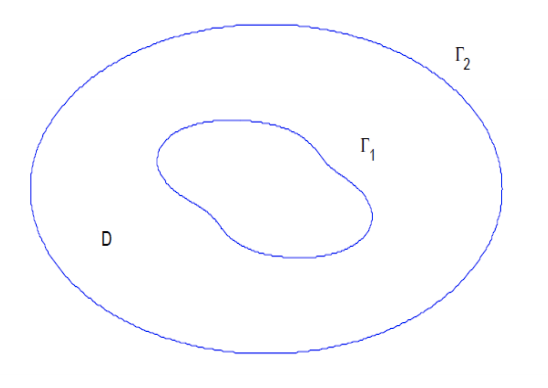
\includegraphics[width=0.5\textwidth]{resources/doubly-connected-region}
		\caption{}
		\label{fig:double-connected-region}
	\end{figure}

	Мішана задача Діріхле-Неймана для рівняння Лапласа полягає в знаходженні такої функції $u(x_1, x_2) \in C^{2}(D) \cup  C^{1}(\overline{D})$ що задовольняє

	\begin{enumerate}
		\item
		Рівняння Лапласа: 
		\begin{equation}
			\Delta{u} = 0 \quad \text{в} \quad D
		\end{equation}

		\item
		Граничні умови:
		\begin{equation}
			\label{dirichlet-condition}
			u = f_1, \quad (x_1, x_2) \in \Gamma_1,
		\end{equation}
	
		\begin{equation}
			\label{neumann-condition}
			\pdv{u}{v} = f_2, \quad (x_1, x_2) \in \Gamma_2 		
		\end{equation}

	\end{enumerate}
	, де $v = v(x)$ - одиничний вектор зовнішньої нормалі, (\ref{dirichlet-condition}) є умовою Діріхле, а (\ref{neumann-condition}) є умовою Неймана.

\end{document}
